\begin{comment}
	\pagebreak
\end{comment}

\section{Recurrent Neural Network}
\textbf{Dyn. System:}$h^t = f(h^{t-1}, x^t; \theta)$\\
\begin{comment}
	The state at time t depends on the state at time t-1.\\
	\Note{We assume here that the same transition function and parameters are used for each timestep, also called auto-regressive models}\\
	
	\begin{Figure}
 		\centering
 		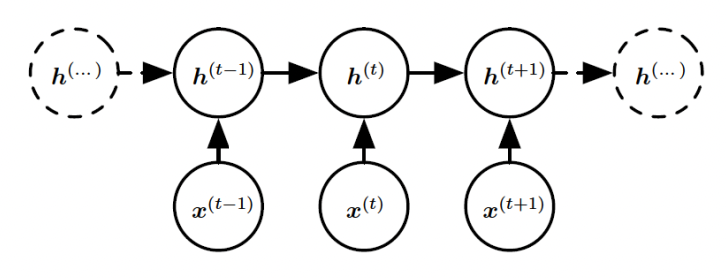
\includegraphics[width=\linewidth]{graphic/rnn-unrolled}
 		\captionof{figure}{Visualisation unrolled RNN}
	\end{Figure}
	\begin{Figure}
 		\centering
 		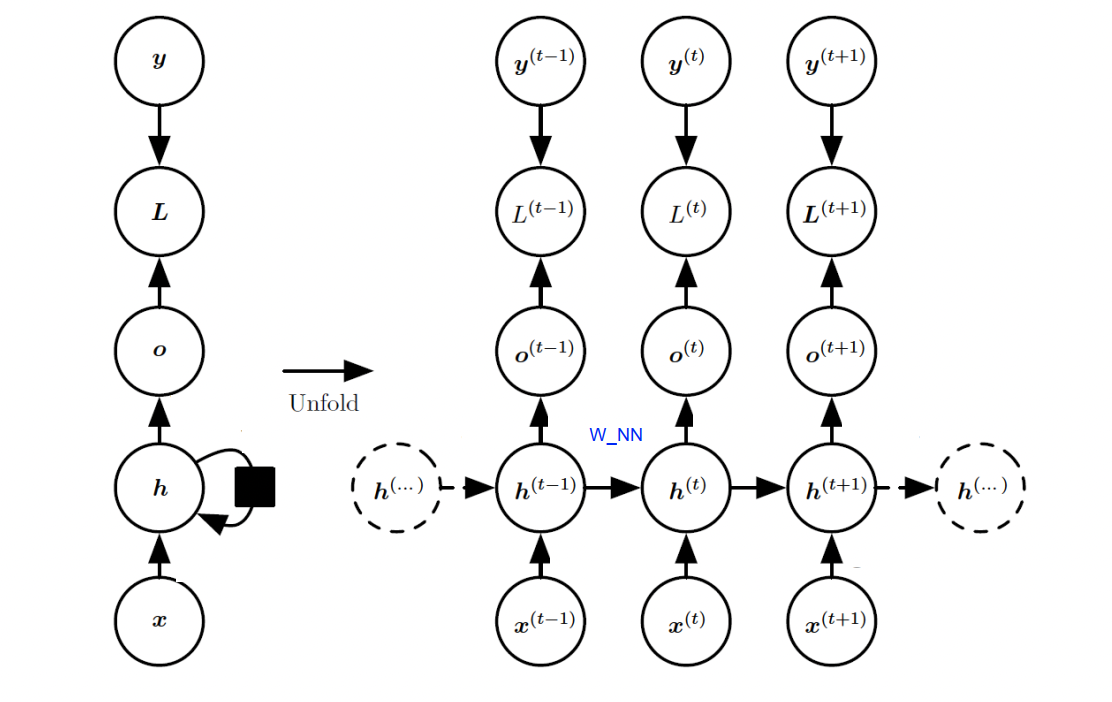
\includegraphics[width=\linewidth]{graphic/rnn-detailed}
 		\captionof{figure}{Visualisation of complex RNN}
	\end{Figure}
\end{comment}

\textbf{Vanilla RNN:} $\why = W_{hy} h^t$, $h^t = tanh(W_{hh} h^{t-1} + W_{xh} x^t)$
\begin{comment}
	\begin{Figure}
 		\centering
 		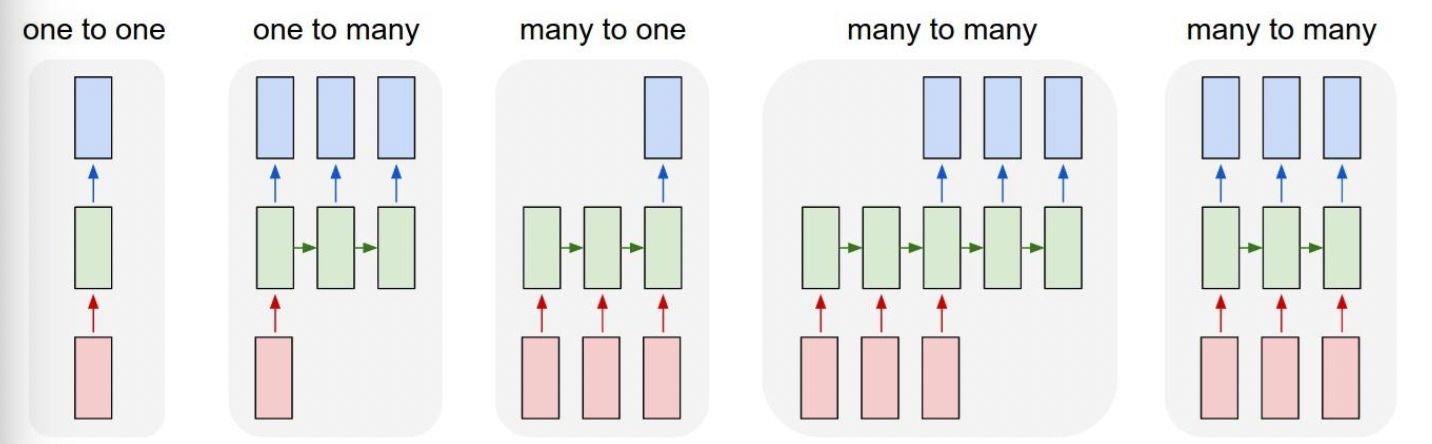
\includegraphics[width=\linewidth]{graphic/rnn-systems}
 		\captionof{figure}{Possibilities of RNN architectures}
	\end{Figure}
\end{comment}

\textbf{Backprop:} $h^t = f(h^{t-1}, x^t; W), 
\why^t = W_{hy}h^t, 
L^t = \norm{\why^t - y^t} ^2,
\frac{\delta L}{\delta W} = \sum_{t=1}^S \frac{\delta L^t}{\delta W}$\\
\begin{comment}
	Treat unrolled recurrent modelas multi-layer Network with unbounded number of layers and perform backprop.\\
	
	\begin{Figure}
 		\centering
 		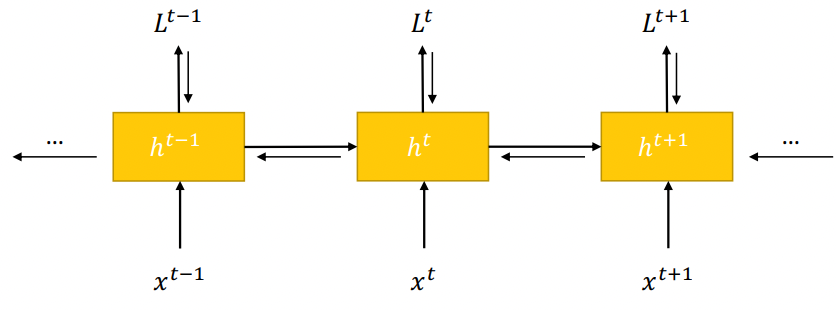
\includegraphics[width=\linewidth]{graphic/rnn-backprop}
 		\captionof{figure}{Unrolling of RNN}
	\end{Figure}
\end{comment}

$\frac{\delta L^t}{\delta W} = \sum_{k=1}^t \frac{\delta L^t}{\delta y^t} \frac{\delta y^t}{\delta h^t} \frac{\delta h^t}{\delta h^k} \frac{\delta^+ h^k}{\delta W}$\\
\begin{comment}
	The $\delta^+$ indicates the immediate loss, since we could take the derivative infinite amount of times (apparently).\\

	\begin{Figure}
 		\centering
 		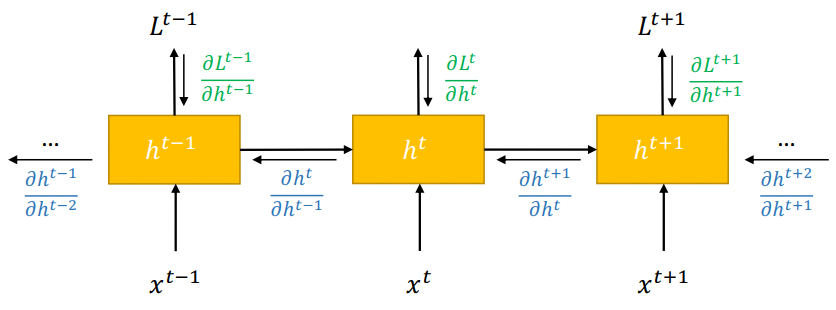
\includegraphics[width=\linewidth]{graphic/rnn-backprop-2}
 		\captionof{figure}{Unrolling of RNN - Individual Loss}
	\end{Figure}
\end{comment}

\textbf{Grads:} $h^t = W^T h^{t-1} = (W^T)^t h^1 = (Q^T \Lambda^t Q) h^1$\\
\begin{comment}
	The Eigenvalues explode or vanish, depending on their initial size.\\
	\Note{Regularizing the Eigenvalues is proven to reduce the learning capabilities of the learning-system drastically.}\\
	
	\begin{Figure}
 		\centering
 		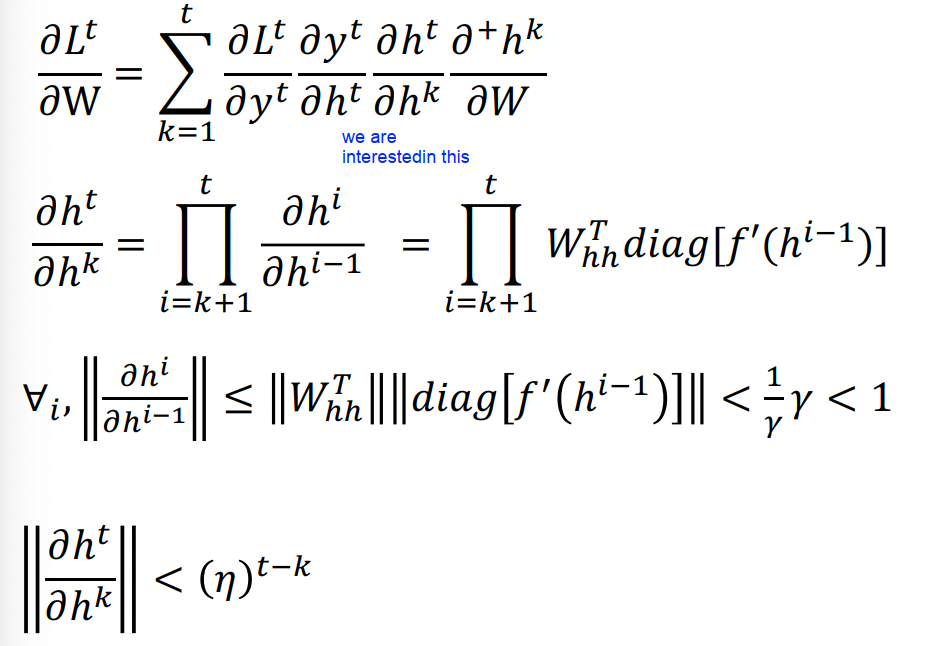
\includegraphics[width=\linewidth]{graphic/rnn-vanishing-gradient-proof}
 		\captionof{figure}{Proof that vanishing Gradients are a problem}
	\end{Figure}
\end{comment}

\textbf{Naive LSTM:} $c_t = Wc^{t-1} + W_g g^t, h^t = tanh(c^t)$\\
\begin{comment}
	\begin{Figure}
 		\centering
 		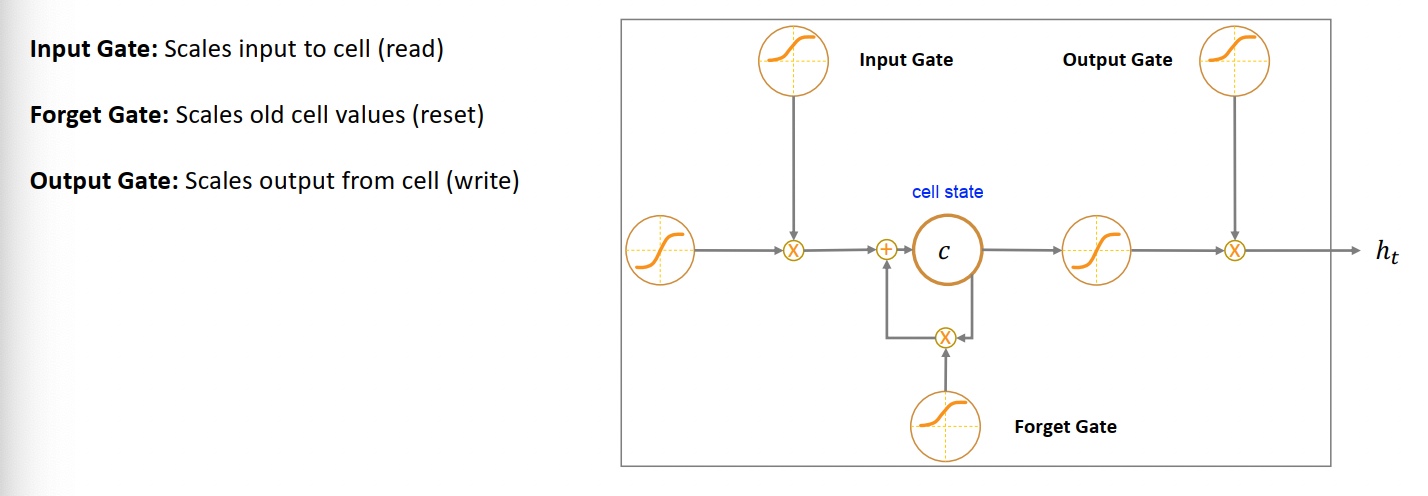
\includegraphics[width=\linewidth]{graphic/rnn-abstract-lstm}
 		\captionof{figure}{LSTM Abstraction}
	\end{Figure}
	\begin{Figure}
 		\centering
 		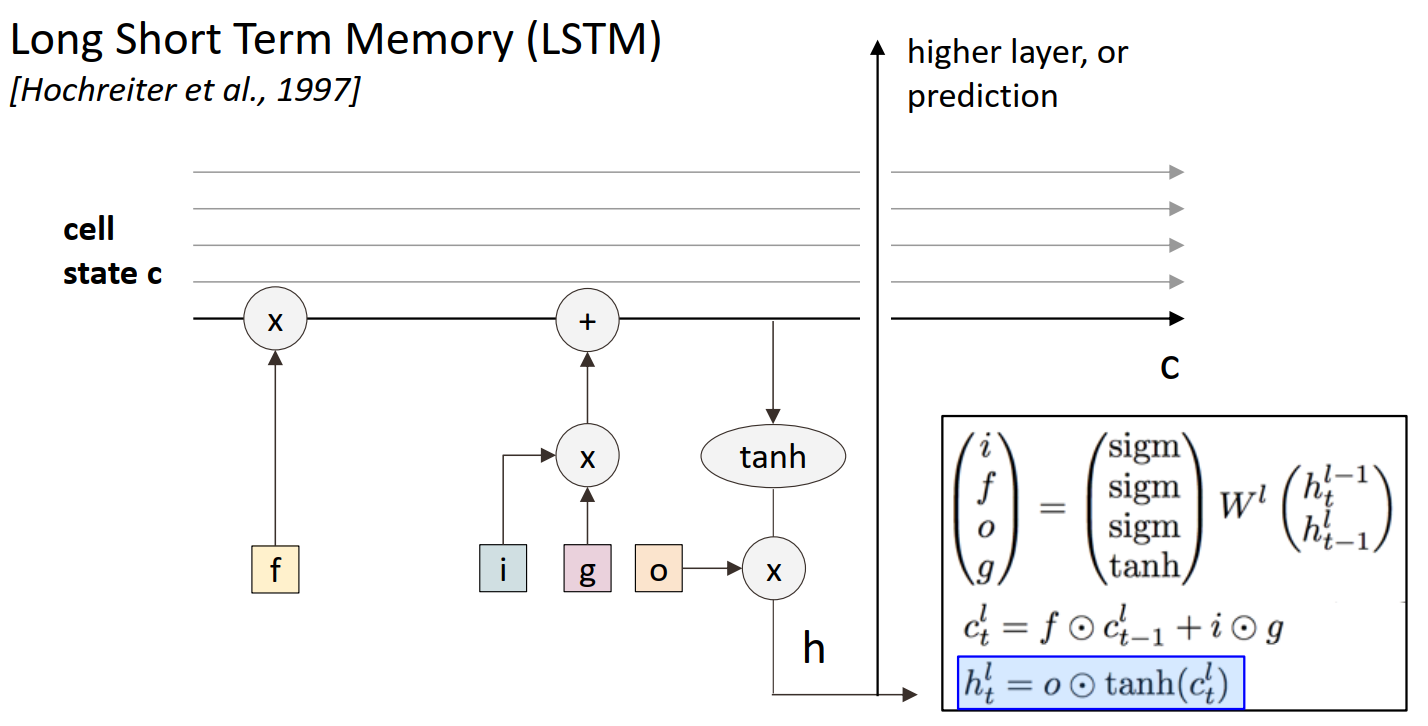
\includegraphics[width=\linewidth]{graphic/rnn-lstm}
 		\captionof{figure}{LSTM Visualization}
	\end{Figure}
	\begin{Figure}
 		\centering
 		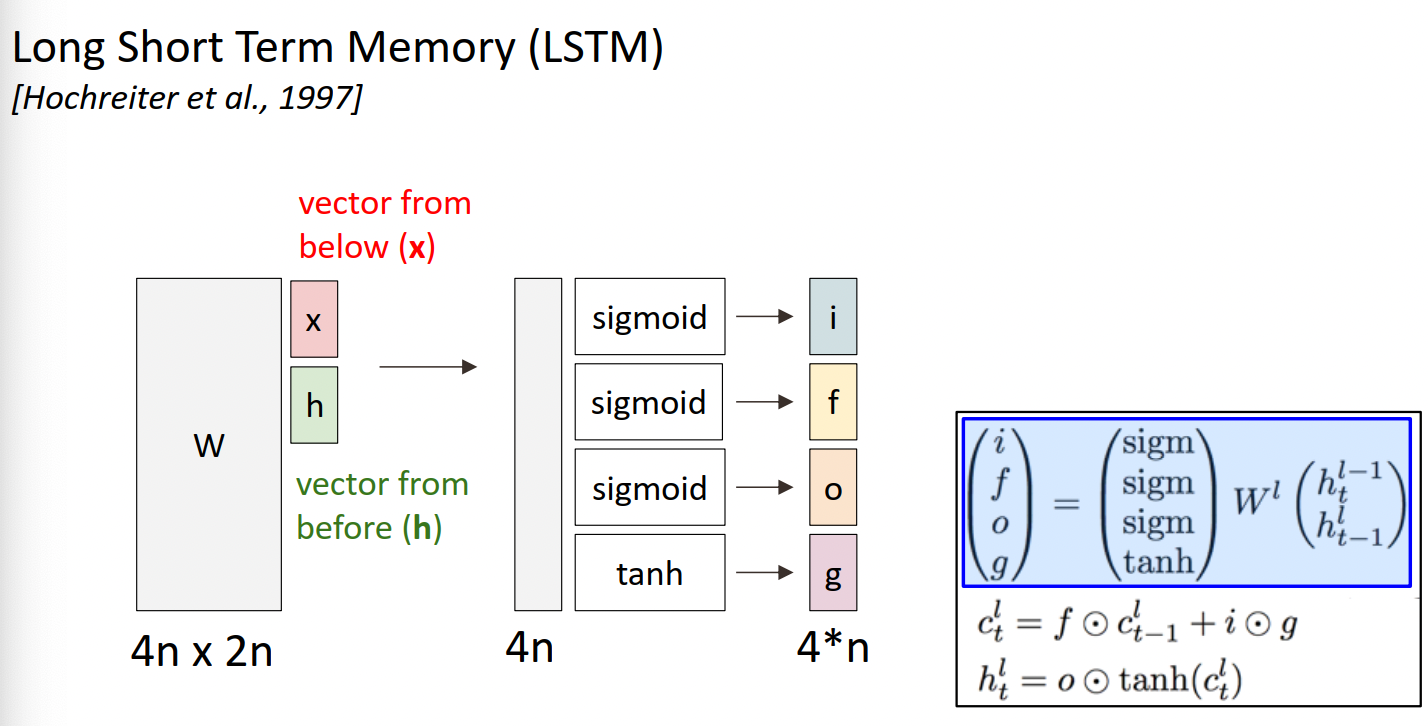
\includegraphics[width=\linewidth]{graphic/rnn-lstm-2}
 		\captionof{figure}{LSTM Visualization}
	\end{Figure}
\end{comment}
\question{How does this work?}\\
\todo{Calculate through the matrices and functions to see if it works}\\

\textbf{RNN vs. LSTM:} memory cell, adding gradient to stabalize\\
\begin{comment}
\begin{Figure}
 		\centering
 		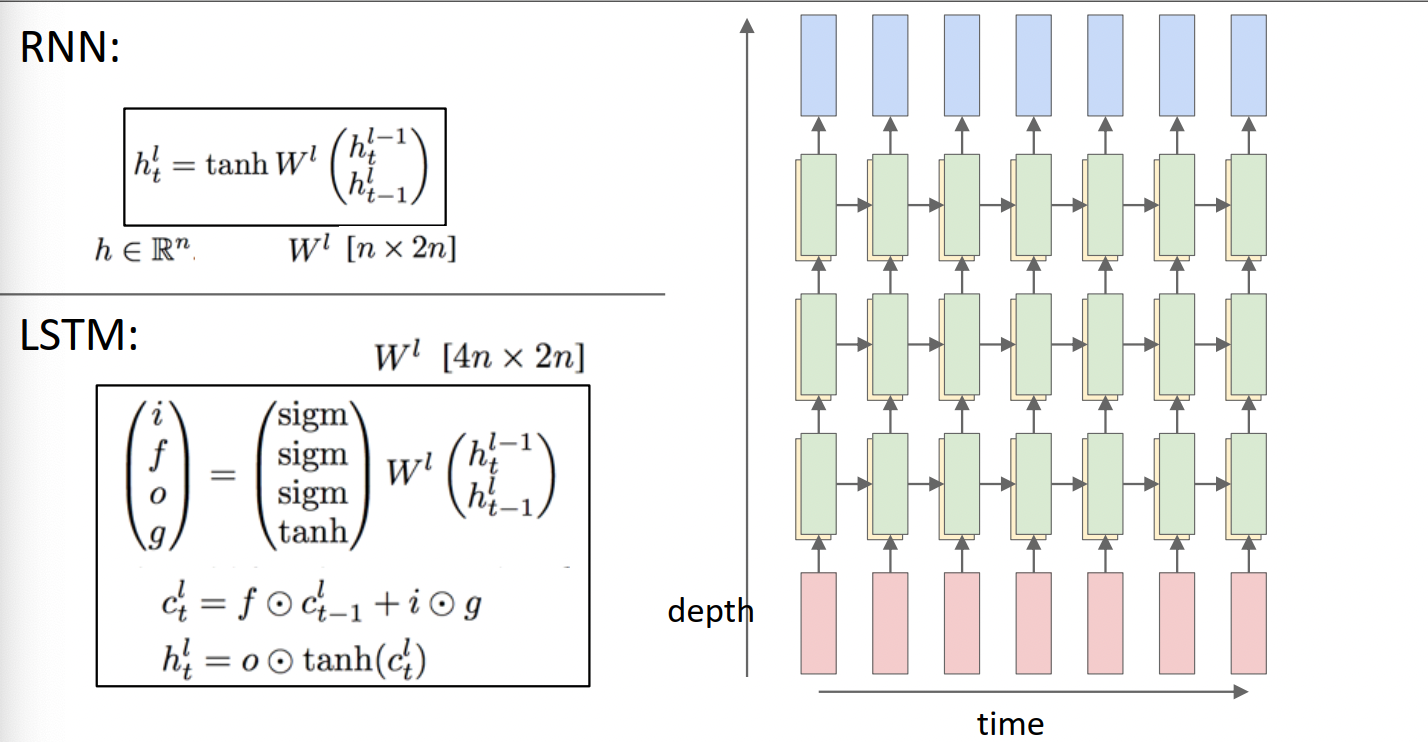
\includegraphics[width=\linewidth]{graphic/rnn-vs-lstm-2}
 		\captionof{figure}{LSTM vs. RNN}
	\end{Figure}
	\begin{Figure}
 		\centering
 		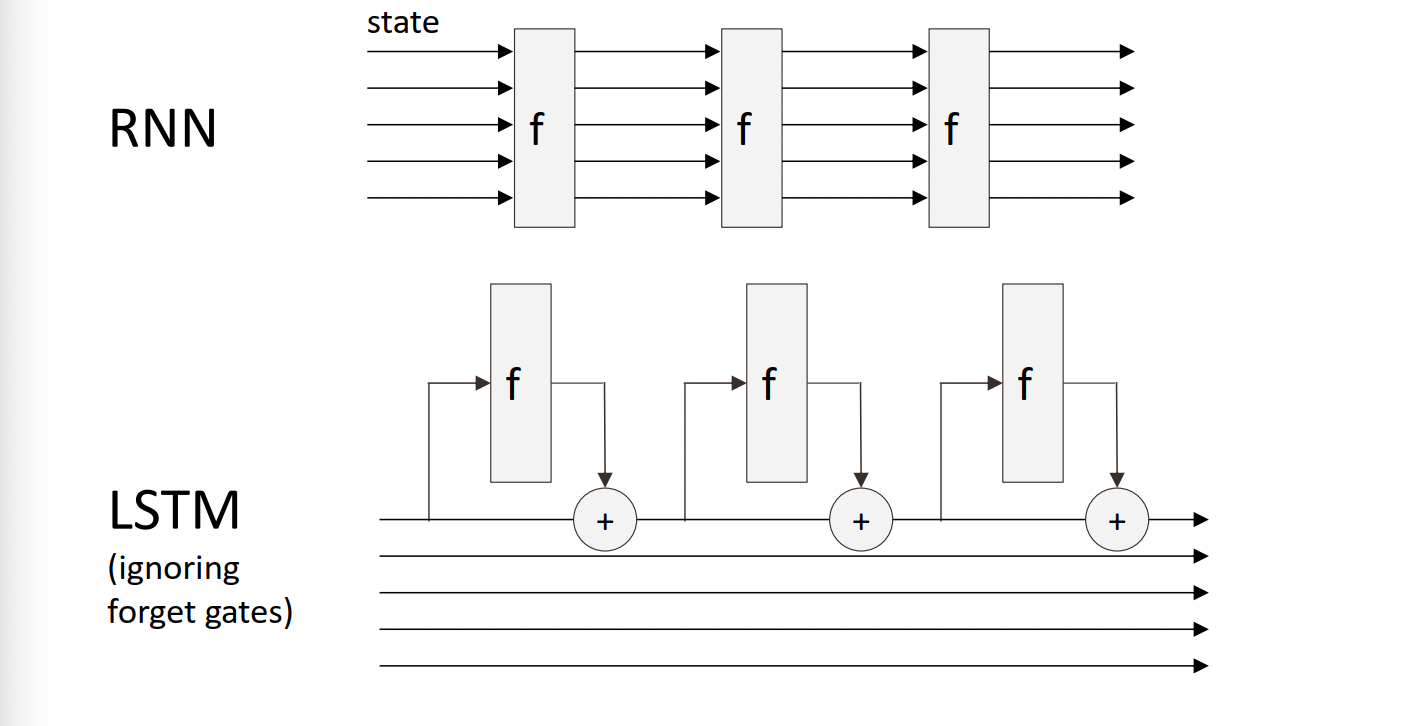
\includegraphics[width=\linewidth]{graphic/rnn-vs-lstm-1}
 		\captionof{figure}{LSTM vs. RNN}
	\end{Figure}
\end{comment}

\textbf{Grad. clipping:} Clip gradient, don't allow big jumps\\
\begin{comment}
	When the gradient gets too big the learning gets unstable, because the big gradient allows huge jumping around.
	Clipping it might reduce the performance, but at least the direction is more stable.\\
\end{comment}




